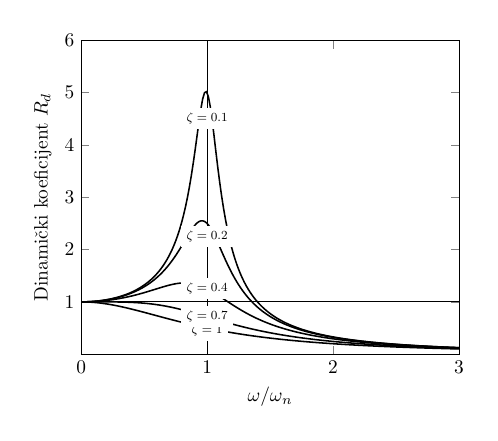
\begin{tikzpicture}[scale=0.7]
    \begin{axis} [
        ylabel = Dinamički koeficijent $R_d$,
        xlabel = $\omega/\omega_n$,
        xmin = 0, xmax = 3,
        ymin = 0, ymax = 6,
        xtick = {0, 1, 2, 3},
        ytick = {1, 2, 3, 4, 5, 6},
     ]

        \draw[thin] (1,0) -- (1,6);
        \draw[thin] (0,1) -- (3,1);
    \foreach \i in {1, 0.7, 0.4, 0.2, 0.1}
        {
            \addplot [
                domain=0:3,
                samples=200,
                color=black,
                thick,
            ]{1/((1-x^2)^2+(2*\i*x)^2)^0.5};
        }
    \pgfplotsinvokeforeach{1, 0.2, 0.1}
        {
            \node[rectangle,fill=white,scale=0.8] at 
                (1,{(1-0.1)/(2*#1)}) {\footnotesize{$\zeta=#1$}};
        }
    \pgfplotsinvokeforeach{0.7, 0.4}
        {
            \node[rectangle,fill=white,scale=0.8] at 
                (1,{1/(2*#1)}) {\footnotesize{$\zeta=#1$}};
        }

    \end{axis}
\end{tikzpicture}
